% Activate the following line by filling in the right side. If for example the name of the root file is Main.tex, write
% "...root = Main.tex" if the chapter file is in the same directory, and "...root = ../Main.tex" if the chapter is in a subdirectory.
 
%!TEX root =  testMain.tex

\chapter[Simple Non-Spatial Simulations]{A Simple Stabbing - Non-Spatial Simulations and their Bayesian Networks}

\section{Introduction}

This first experiment is not a true agent model. Agents have, as their name suggest, a limited amount of agency. They have knowledge and can interact with the world and each other. This simulation does not contain agents and is instead based on simple rule-based inference.

This chapter is meant to show that we can:
\begin{itemize}
\item create a simulation that runs on an uncertain rule-based inference engine. 
\item create reporters that capture the state of the simulation.
\item the output of the reporters can be used to automatically generate Bayesian Networks.
\item we can apply our performance criteria to these Bayesian Networks.
\end{itemize}

Apart from these goals, we will then also compare the networks to the networks created in \citet{Vlek2015}. If we find that our method functions well, then we have a chance to apply it to complex spatial simulations in the following chapters. If we cannot make BNs out of this simple simulation, then the rest of our endeavour will be fruitless.

\section{Method}
%There are two methods outlined here, one for each initial experiment.
We want to see if our method can produce similar Bayesian Networks as those in \citet{Vlek2015}. This means that we take the two scenarios presented in that paper as inspiration. The facts that both scenarios agree on, are these: Jane and Mark had a fight, and Jane had a knife. Something Happened, and then Mark died. 

The problem here, is that Something Happened. The two scenarios that explain why Mark died, are

Scenario 1, Jane stabbed Mark, and then he died. 

Scenario 2, Jane threatened Mark with the knife, Mark hit Jane, Jane dropped the knife, Mark fell on the knife, and Mark died by accident. 

These two scenarios are represented by two different Bayesian networks (Figure~\ref{vlek1} and Figure~\ref{vlek} for replications of the Bayesian Network structure for scenario 1 and 2 respectively). In \citet{Vlek2015}, no probabilities are given, as this paper considers how the structure of the networks represents completeness, consistency and plausibility, and is not meant as an investigation into probability elicitation.

For this experiment, every fact \footnote{Or event, or random variable, or reporter, these are all interchangible in this chapter.} that is represented in the network, is represented as a fact in an uncertain forward chaining inference engine. We are creating a simulation using this engine (this is our data-generating environment). We are creating 3 different simulations: one for scenario 1, another for scenario 2, and a third for a combination, where either scenario 1 happens, or scenario 2, but we do not know which. The output of these simulations is presented to the K2 algorithm, which builds us Bayesian Networks that we can then evaluate.

The uncertain forward chaining engine is the simulation. Every fact has a prior probability, and every conclusion of a rule has a probability given the state of the premises. At every step, the simulation checks which new sentences are true, applies a rule with a given probability, and counts the outcome using the reporters of the same name with the process outlined in the previous chapter.

\subsection{Behavioural rules for the simulation}

\begin{table}
\begin{tabular}{|c|c|c|}
 \hline
 Premise & Conclusion & P(conclusion) given premises\\
 \hline
  & Jane and Mark fight   & 20   \\
  & Jane has knife & 70 \\
  \color{blue}Jane and Mark fight, Jane has a knife & Jane stabs Mark with knife & 1 \\
 \color{red}Jane and Mark fight, Jane has a knife & Jane threatens Mark with knife & 3 \\
  \color{red}Jane threatens Mark with knife & Mark hits Jane & 90 \\
  \color{red}Mark hits Jane & Jane drops knife & 50  \\
  \color{red}Jane drops knife & Mark falls on knife & 10 \\
  \color{red} Mark falls on knife & Mark dies by accident & 60  \\
  \color{blue}Jane stabs Mark with knife & Mark dies  & 70 \\ 
  \color{red}Mark dies by accident & Mark dies & 100  \\ 
\hline
\end{tabular}
\caption{For combined scenarios: blue rules belong to scenario 1, red rules belong to scenario 2, and black rules belong to both.}
\end{table}

This was done using forward chaining, with a time index, which means that a rule could only be triggered at one time (otherwise the probabilities get messed up). So we have a forward chaining rule, which means that if the premises of some rule are true, there are no excluding facts true, the timestep is correct, and the random number generator generated a number that is lower than the probability threshold, we find that the conclusion is true, and add it to our found facts, until we cannot generate any new facts anymore.

The probabilities for these rules to fire were chosen as by the modeller as a subjective estimation of how often these events `might happen', and do not correspond to real statistics. Each simulation was run 50,000 times.


\section{Results}
We succeeded in generating three different BNs, one per scenario (Figure~\ref{kb1}, Figure~\ref{kb2}, Figure~\ref{full}, with the networks from \citet{Vlek2015} on the side for comparison).

\begin{figure}[htbp]
\begin{subfigure}{.4\textwidth}
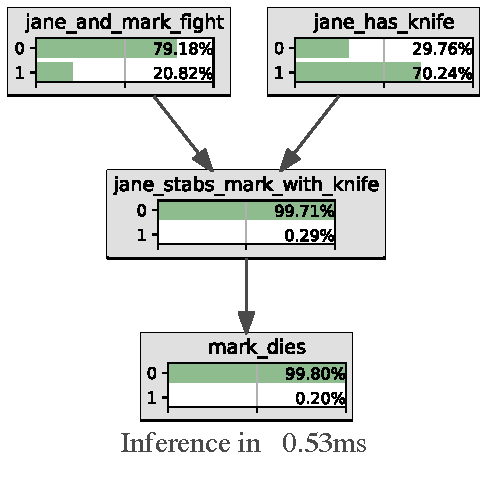
\includegraphics[width=\linewidth]{../experiments/VlekNetwork/bnImage/BNIMAGEKB1.pdf}
\caption{Automatically generated.}
\label{kb1}
\end{subfigure}
\begin{subfigure}{.6\textwidth}
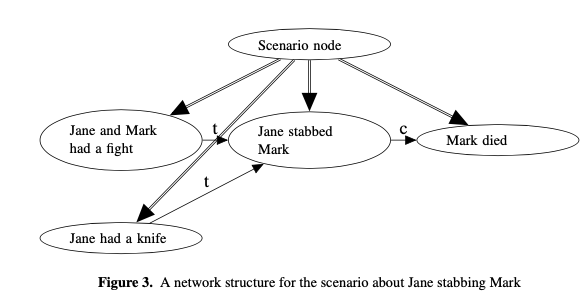
\includegraphics[width=\linewidth]{images/vlek2015a.png}
\caption{Original BN.}
\label{vlek1}
\end{subfigure}
\caption{Scenario 1}
\end{figure}


\begin{figure}[htbp]
\begin{subfigure}{.4\textwidth}
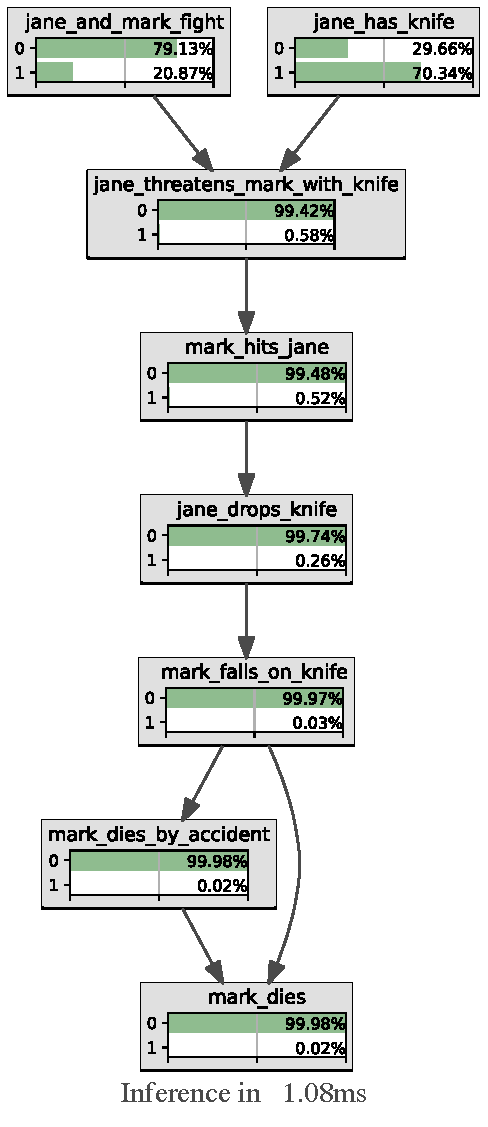
\includegraphics[scale=0.7]{../experiments/VlekNetwork/bnImage/BNIMAGEKB2.pdf}
\caption{Automatic generated.}
\label{kb2}
\end{subfigure}
\begin{subfigure}{.7\textwidth}
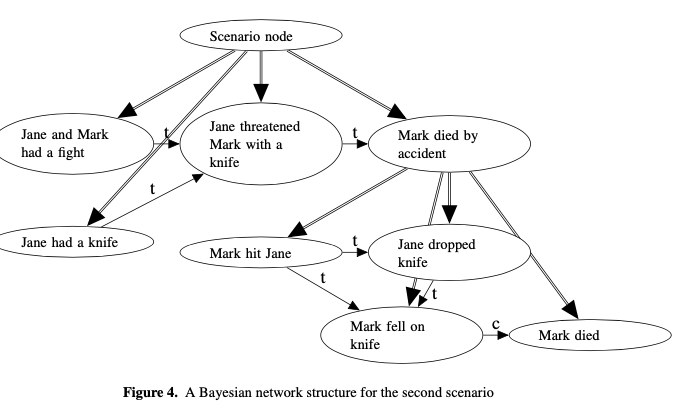
\includegraphics[scale=0.4]{images/vlek2015.png}
\caption{Original BN.}
\label{vlek}
\end{subfigure}
\caption{Scenario 2}
\end{figure}


\begin{figure}[htbp]
\begin{center}
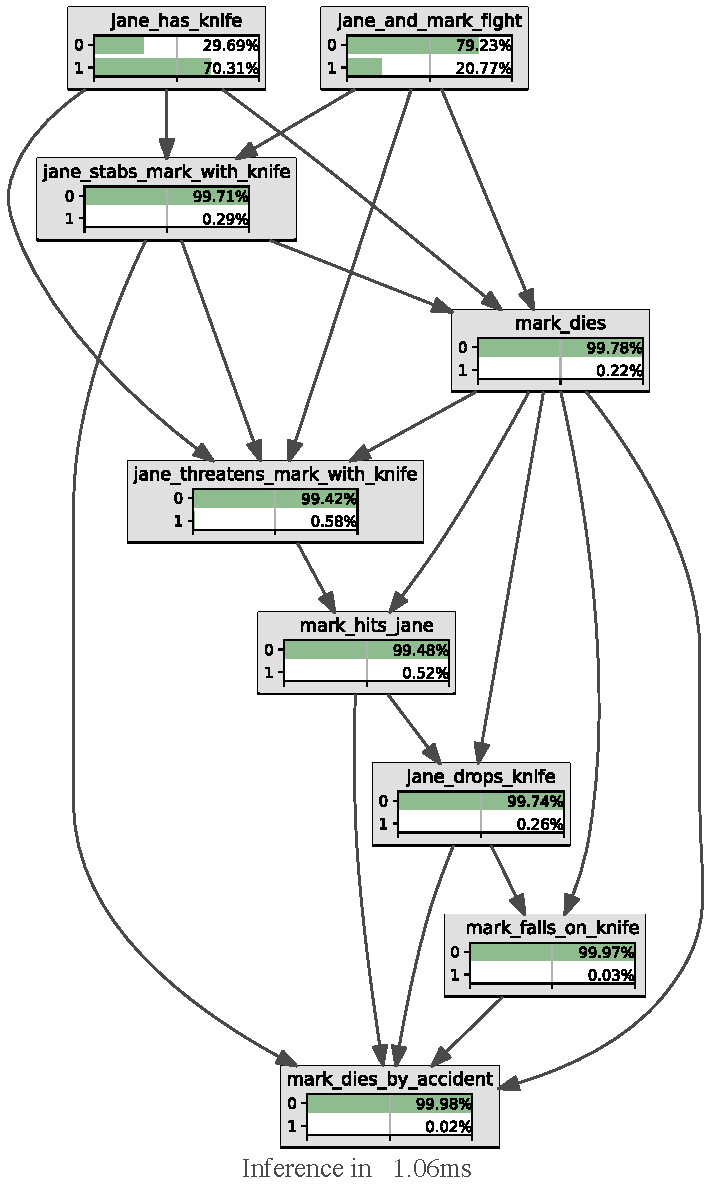
\includegraphics[scale=0.8]{../experiments/VlekNetwork/bnImage/BNIMAGEKBFull.pdf}
\caption{Automatically generated BN with rules from both scenarios included.}
\label{full}
\end{center}
\end{figure}


\subsection{Evaluation with regards to structural, performance and human-factor criteria}
In this section, the evaluation criteria as set out before are applied to the networks.


\subsubsection{Structural Criteria}
\begin{enumerate}
\item \textbf{Hypotheses are ordered temporally.}

We see that in both the separate networks, the temporal ordering of the nodes is correct - every node has as a parent a node that represents an event that would have happened earlier. In the combined network, this is not the case: there are some temporal links - the chain of events from "Jane threatening Mark" to "Mark dies by accident" is represented correctly, however, every node in this chain has as a parent ``Mark dies", which would, temporally, occur only after "Mark falls on knife" occurs.

The combined Bayesian Network brings up difficulties for temporal ordering. If we try to merge two mutually exclusive scenarios, we cannot meaningfully speak of that `Jane stabs Mark' happens before or after `Jane threatens Mark' - either one of these events happen, never both, and no one of them will happen before or after the other. This is not a problem for the performance of the Bayesian Network - we can arbitrarily decide on a parent node, and interpret the arcs as conditional, and not temporal or causal. However, structurally, it is easier to think about the links as temporal, and temporally organised `within' scenarios. 

\item \textbf{Evidence connects to hypotheses.}

In these networks and simulation, no evidence is implemented yet, that means that this criteria does not apply.

\item \textbf{Relevance: All relevant events are in the BN, all irrelevant events are outside of the BN.}
This criteria, and the next one, are freebies, because we are just copying a network that already exist - our set of relevant events is the same as that in the original network by Vlek. By the structure of the network, we see that all events are connected to each other, there is no node that is both without parents and without children, which means that all nodes are relevant in that they represent conditional relations.

\item \textbf{Independent events are not connected to each other.}

This is done correctly in the non-combined networks, where each node has appropriate parents. However, in the combined network, we see that this goes wrong.

\end{enumerate}

\subsubsection{Performance Criteria}
We consider the accuracy and root mean square per network, then also look at the correspondence, sensitivity values and the progression given a certain evidence set.

\begin{enumerate}
\item \textbf{Accuracy and Root Mean Square error}

The accuracy and rmse are shown in Table~\ref{tabA}.

\begin{table}[h]
\begin{center}
\begin{tabular}{|c|c|c|}
 \hline
 Network & Accuracy & Root Mean Square\\
 \hline
 Scenario 1   & 0.83 &  0.17   \\
 Scenario 2 & 0.88 & 0.14 \\
 Combined & 0.81 & 0.2 \\
\hline
\end{tabular}
\caption{Accuracy and Root Mean Square Error for the networks}
\label{tabA}
\end{center}
\end{table}

\item \textbf{Correspondence.}

In this case, we know exactly the frequencies of events given their premises in the rule base, because we have set them explicitly in our probabilistic-forward-chaining engine. These frequencies are represented in Table~4.5 as the `True P(event)' column. The `P(event)' column is the result of the prediction of the Bayesian Network. As shown in the tables, the Bayesian Network \textbf{usually} estimates the probability of the event within ±1\% uncertainty. There are a few exceptions to the general behaviour of less than ±1\% uncertainty in the network - the network generally overestimates small probabilities. Whether an uncertainty of `generally less than ±1\%' is good or bad depends on the precision that the network requires - since we do not have any evidence that really depends on high-precision data or networks (eg: a change of 0.01 in one node results in a different conclusion - see sensitivity analysis and precision reduction), the Bayesian Networks seems satisfactory. 


\begin{table}
\begin{center}
\begin{tabular}{|c|c|c|}
 \hline
 Conclusion & True P(event) & P(event) \\
 \hline
 Jane and Mark fight   & 20 &  20.87   \\
 Jane has knife & 70 & 70.23 \\
 Jane stabs Mark with knife & 1 & 2.05 \\
 Mark dies & 70 & 75.46 \\ 
\hline
\end{tabular}
\caption{For only scenario 1.}

\begin{tabular}{|c|c|c|}
 \hline
 Conclusion & True P(event) & P(event)\\
 \hline
 Jane and Mark fight   & 20 &  20.87   \\
 Jane has knife & 70 & 70.23 \\
 Jane threatens Mark with knife & 3 & 3.88 \\
 Mark hits Jane & 90 & 90.21 \\
 Jane drops knife & 50 & 50.09 \\
 Mark falls on knife & 10 & 11.13\\
 Mark dies by accident & 60 & 61.25 \\
 Mark dies & 100 & 99.79 \\ 
\hline
\end{tabular}
\caption{For only scenario 2}

\begin{tabular}{|c|c|c|}
 \hline
 Conclusion & True P(event) & P(event)\\
 \hline
 Jane and Mark fight   & 20 &  20.87   \\
 Jane has knife & 70 & 70.17 \\
 Jane stabs Mark with knife & 1 & 2.06 \\
 Jane threatens Mark with knife & 3 & 3.88 \\
 Mark hits Jane & 90 & 91.50 \\
 Jane drops knife & 50 & 52.97 \\
 Mark falls on knife & 10 & 10.92\\
 Mark dies by accident & 60 & 66.33 \\
 Mark dies (premise: Jane stabs Mark) & 70 & 68.68 \\ 
  Mark dies (premise: Mark dies by accident)& 100 & 98.77 \\ 
\hline
\end{tabular}
\label{test}
\caption{For combined scenarios}
\end{center}
\end{table}



\item \textbf{Sensitivity analysis} (Figure~\ref{sa1}, ~\ref{sa2}, ~\ref{sa3}) shows that no irrelevant event influences some output, as well as being robust, as the largest sensitivity values remain smaller than 1. The sensitivity values for the second scenario in the full network are almost insignificantly small, showing that they have very little influence over the `mark\_dies' node.

\begin{figure}[htbp]
\begin{center}
\begin{subfigure}{.33\textwidth}
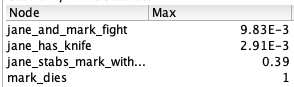
\includegraphics[width=0.9\linewidth]{images/sensitivityKB1.png}
\caption{Sensitivity values for scenario 1 network.}
\label{sa1}
\end{subfigure}%
\begin{subfigure}{.33\textwidth}
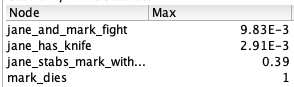
\includegraphics[width=0.9\linewidth]{images/sensitivityKB1.png}
\caption{ Sensitivity values for scenario 2 network.}
\label{sa2}
\end{subfigure}%
\begin{subfigure}{.33\textwidth}
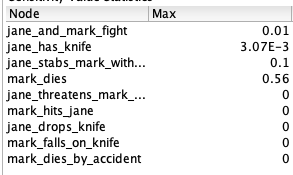
\includegraphics[width=0.9\linewidth]{images/sensitivityKBFull.png}
\caption{Sensitivity values for combined network.}
\label{sa3}
\end{subfigure}
\end{center}
\caption{Sensitivity Analysis}
\label{sa}
\end{figure}

From these values we can see that a parameter chance in most nodes will not affect the output probability very much. The parent nodes of the output node are, of course, the most influential. 


\item \textbf{Effect of evidence on the posterior.}

We plot the effect of a sets of evidence on the posterior (Figure~\ref{kb1a}, ~\ref{kb2a}, ~\ref{fulla}). In each, we select a different story: 

For the first case, Jane has a knife, and Jane and Mark have a fight, but then Jane does not stab Mark - hence, we see the posterior of `mark dies' increase once we learn that they have a fight, and decrease when Jane does not stab Mark.

For the second case, Jane and Mark fight, and Jane has a knife, and Jane threatens Mark with a knife, Mark responds by hitting Jane, and Jane drops the knife. All of these facts cause the posterior of `mark dies' to increase, since, given all of these factors, we would expect it a bit more likely that Mark dies. However, it is a very small increase, from 0.0 to perhaps 0.1. Then, once we learn that Mark actually does fall on a knife, we see the posterior probability of Mark dying increase by much more, growing to 0.5. However, Mark gets lucky, and does not die accidentally (he probably fell on the good side of the knife). Now, the posterior for `mark dies' also goes to 0, since the only way that Mark dies in this scenario is due to an accidental death by falling on a knife. 

The combined scenario represents the story where Jane and Mark fight, Jane has a knife, but Jane does not stab, but threatens instead. Then Mark hits Jane, and Jane drops the knife, which is the highest posterior probability for `mark dies' in the entire story. Then, Mark does not fall on the knife, and Mark does not die by accident, and hence the posterior for `mark dies' goes to 0.

\begin{figure}[htbp]
\begin{subfigure}{.5\textwidth}
 \centering
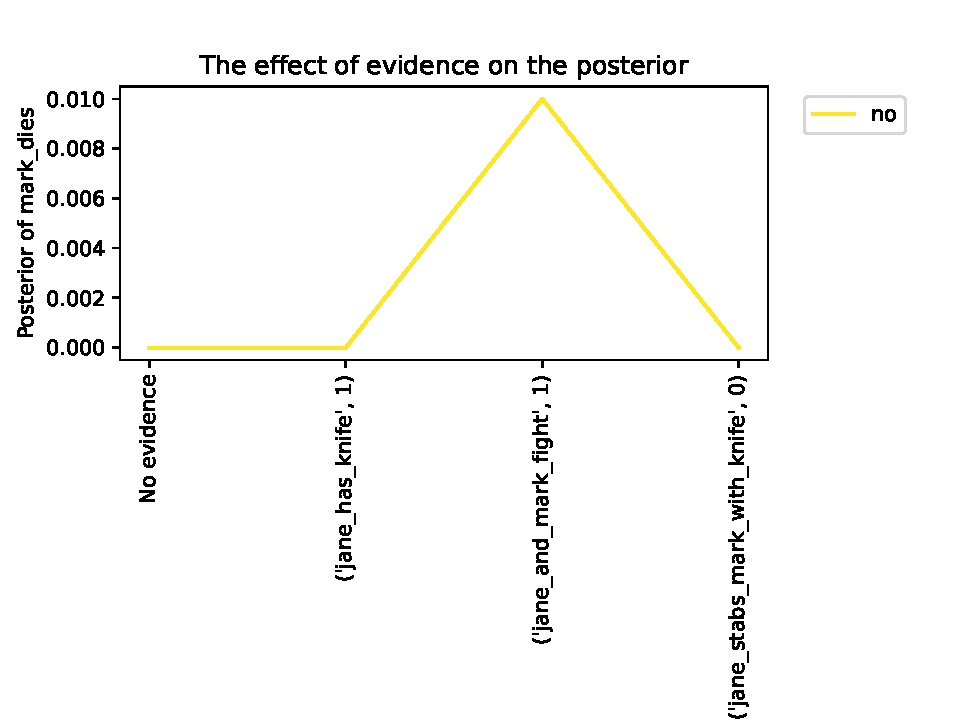
\includegraphics[width=0.95\linewidth]{../experiments/VlekNetwork/plots/posterior_base_networkKB1.pdf}
\caption{ network 1.}
\label{kb1a}
\end{subfigure}%
\begin{subfigure}{.5\textwidth}
\centering
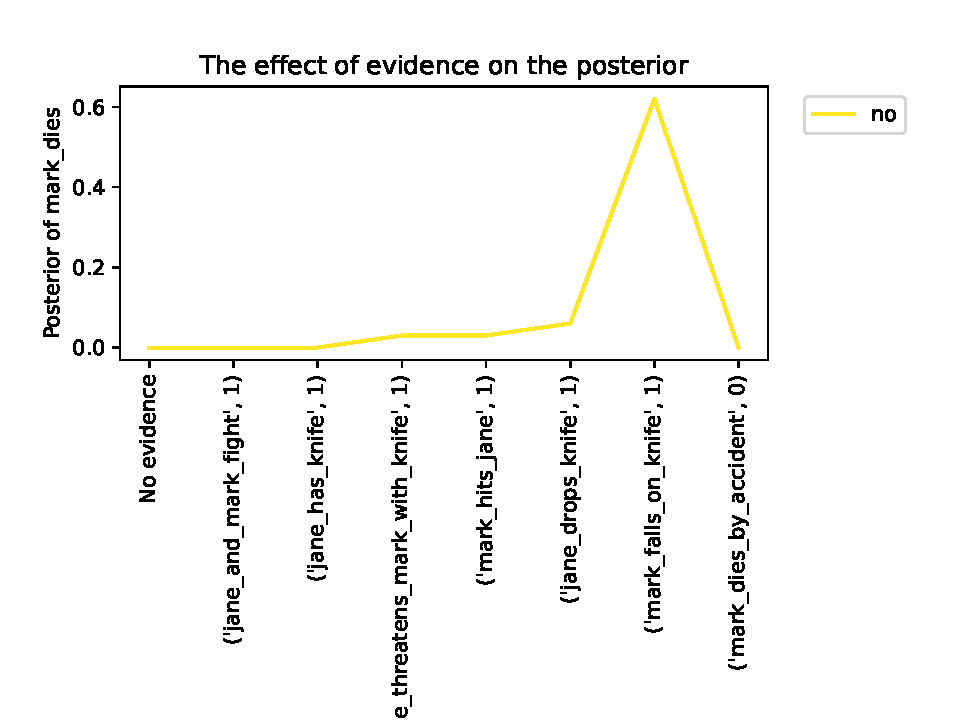
\includegraphics[width=0.95\linewidth]{../experiments/VlekNetwork/plots/posterior_base_networkKB2.pdf}
\caption{ network 2.}
\label{kb2a}
\end{subfigure}


\begin{subfigure}{.5\textwidth}
\centering
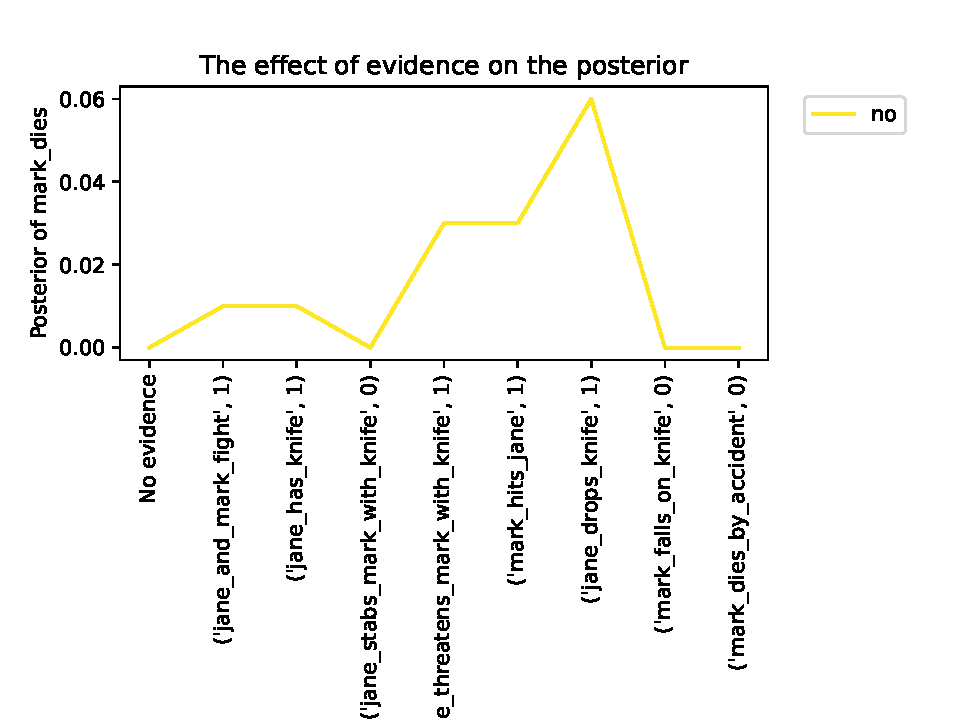
\includegraphics[width=0.95\linewidth]{../experiments/VlekNetwork/plots/posterior_base_networkKBFull.pdf}
\caption{Combined network.}
\label{fulla}
\end{subfigure}
\caption{Posteriors}
\end{figure}

\end{enumerate}

\subsubsection{Human Criteria}
\begin{enumerate}


\item \textbf{How robust is the network against a loss of precision?}

We tested this by changing the cpts to be less and less precise, and plotted the results in Figure~\ref{kb1a1} - ~\ref{fullp}. We can see that the results are very drastic. At around a loss of precision of 0.05 (less for the combined network), the accuracy of the predictions drops from around 80\% to 0\%. 

This dramatic is altogether due to entering inconsistent evidence inside the networks. For example, in the rounded to 0.05 network of the first scenario, trying to add `jane\_stabs\_mark\_with\_knife' as being true, results in the network failing. This is not due to the `mark\_dies' node, but instead due to rounding away to 0 and 1 in the cpt table for `jane\_stabs\_mark\_with\_knife' (Table~\ref{stab}). Entering the evidence that Jane did stab Mark is inadmissible according to the CPT, hence the failed state.

\begin{table}
\begin{center}
\begin{tabular}{|c|c|c|c|c|}
 \hline
 Jane and Mark fight & 1 & 1 &0 & 0 \\
 \hline
 Jane has knife & 1 & 0 &1 & 0 \\
 \hline
 \hline
  P(jane\_stabs\_mark\_with\_knife) & 0 & 0 &0 & 0 \\
  \hline
\end{tabular}
\caption{CPT of jane\_stabs\_mark\_with\_knife}
\label{stab}
\end{center}
\end{table}

But what if we do not round to 0 and 1, but round to $\epsilon$ and $1 - \epsilon$. Here $\epsilon$ would be an approximation of 0 and 1, just purely meant to `unblock' the inference in the Bayesian Networks: going from `never possible' to `not impossible'. If it worked, it would be a pragmatic solution. Hence, the rounding algorithm was adapted to use $\epsilon = 0.01$ - all values that were previously rounded to 1 are instead now 0.99 and all 0's become 0.01.

This intervention is successful. Figure~\ref{error} shows the accuracy of networks under lower and lower degrees of precision, but now rounding to $\epsilon$. We see that after an initial small drop in performance in scenario 2 and the combined scenario, the accuracy of the adjusted networks remains constant at around 80\% in all cases. The only effect we see of the lowered precision is the fact that the RMSE increases slightly as the precision lowers.

\begin{figure}[htbp]
\begin{subfigure}{.5\textwidth}
 \centering
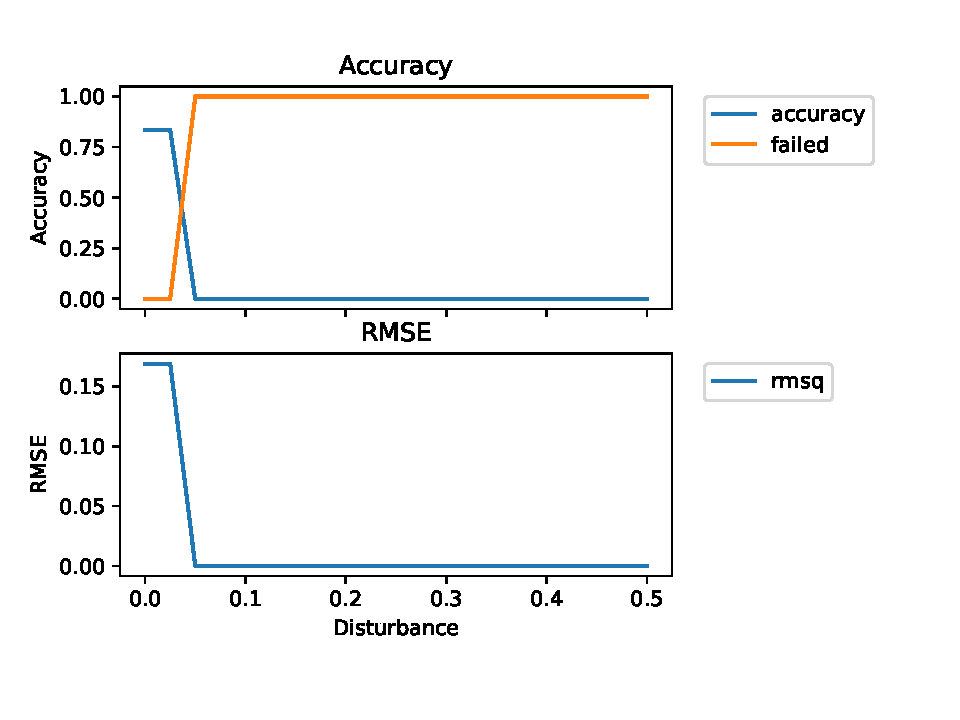
\includegraphics[width=0.9\linewidth]{images/performance_KB1.pdf}
\caption{Network 1 accuracy and RMS.}
\label{kb1a1}
\end{subfigure}%
\begin{subfigure}{.5\textwidth}
 \centering
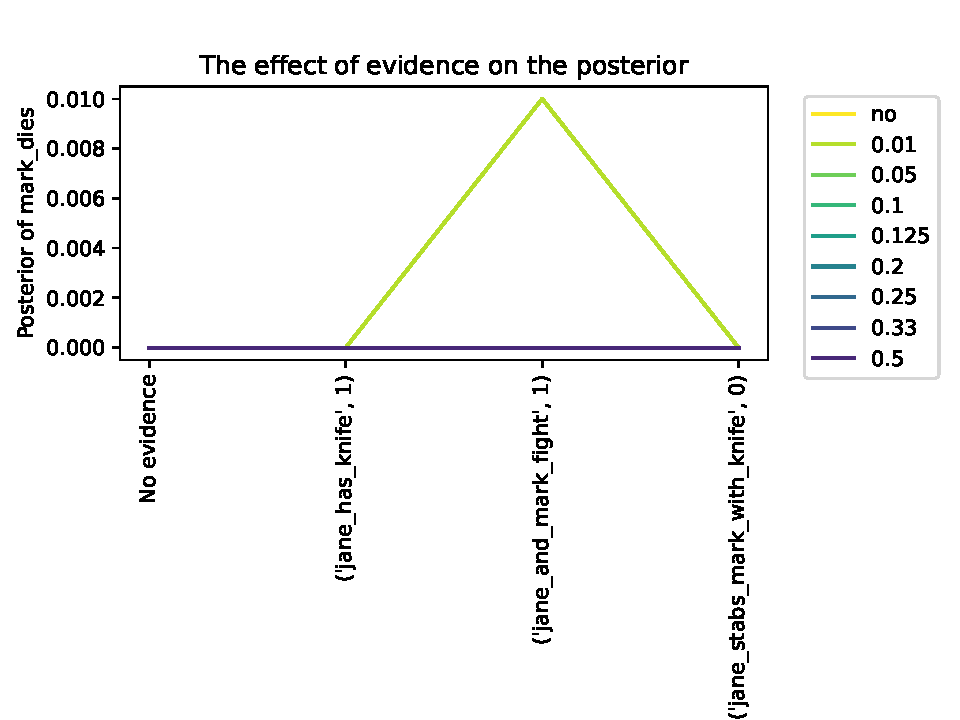
\includegraphics[width=0.9\linewidth]{../experiments/VlekNetwork/plots/posterior_KB1.pdf}
\caption{Network 1 posterior.}
\label{kb1a}
\end{subfigure}
\begin{subfigure}{.5\textwidth}
\centering
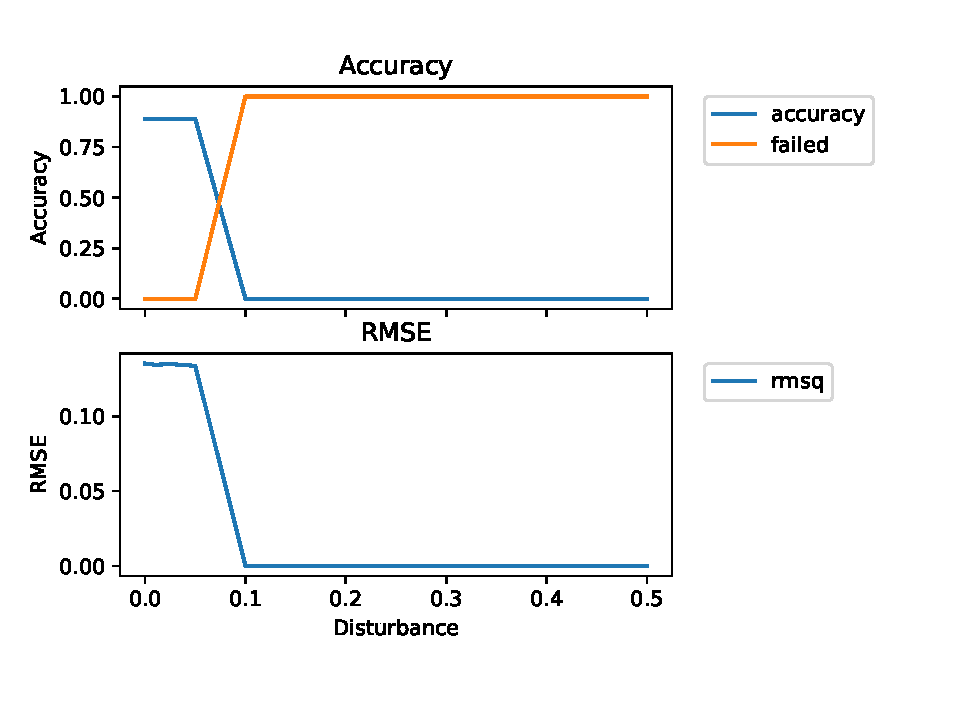
\includegraphics[width=0.9\linewidth]{images/performance_KB2.pdf}
\caption{Network 2 accuracy and RMS.}
\label{kb2a1}
\end{subfigure}%
\begin{subfigure}{.5\textwidth}
 \centering
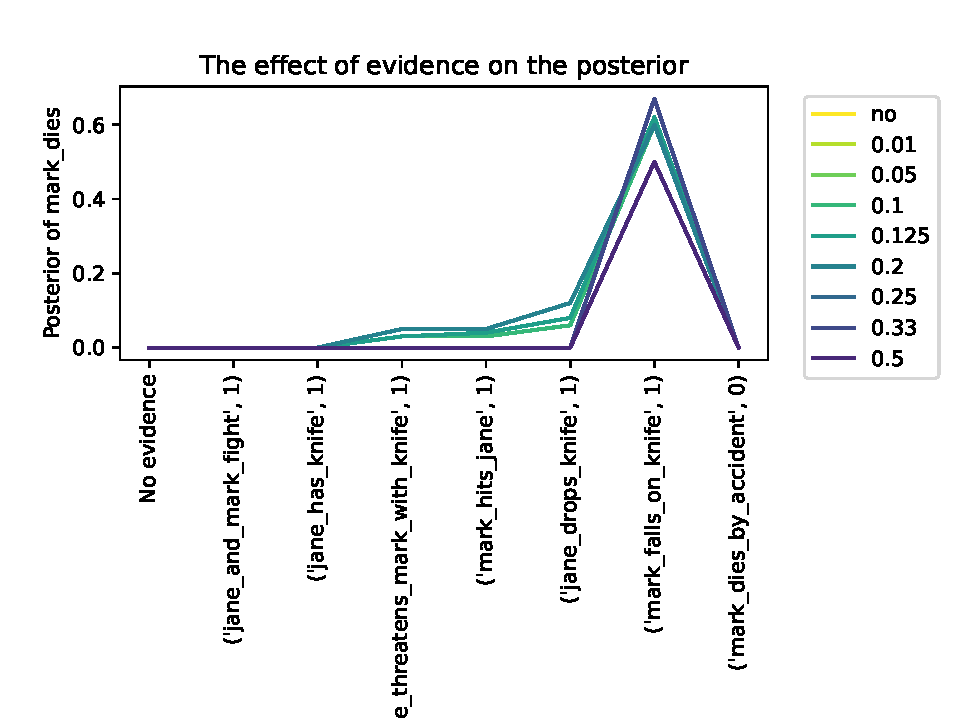
\includegraphics[width=0.9\linewidth]{../experiments/VlekNetwork/plots/posterior_KB2.pdf}
\caption{Network 2 posterior.}
\label{kb2p}
\end{subfigure}

\begin{subfigure}{.5\textwidth}
\centering
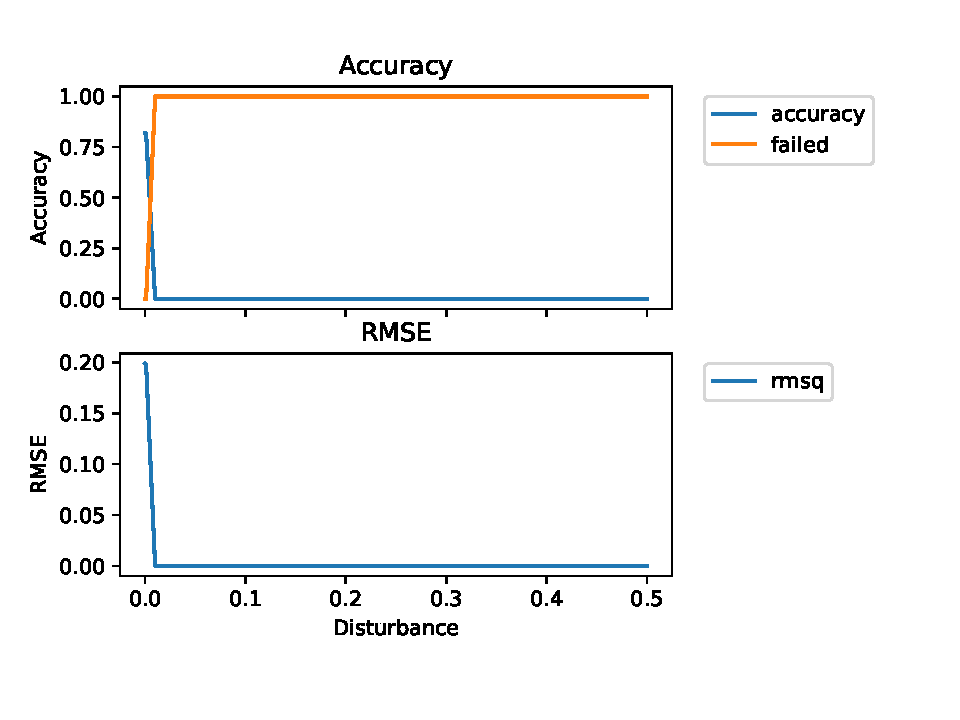
\includegraphics[width=0.9\linewidth]{images/performance_KBFull.pdf}
\caption{Combined network accuracy and RMS.}
\label{fulla1}
\end{subfigure}%
\begin{subfigure}{.5\textwidth}
 \centering
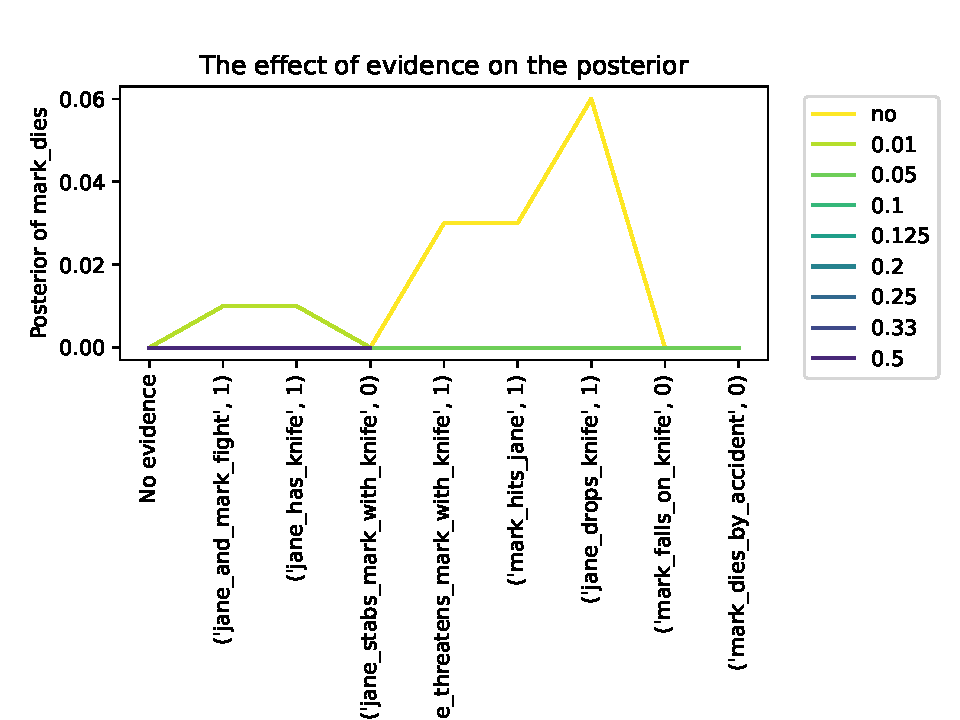
\includegraphics[width=0.9\linewidth]{../experiments/VlekNetwork/plots/posterior_KBFull.pdf}
\caption{Combined network posterior.}
\label{fullp}
\end{subfigure}
\caption{Performance of networks}
\end{figure}

\begin{figure}[htbp]
\begin{subfigure}{.5\textwidth}
\centering
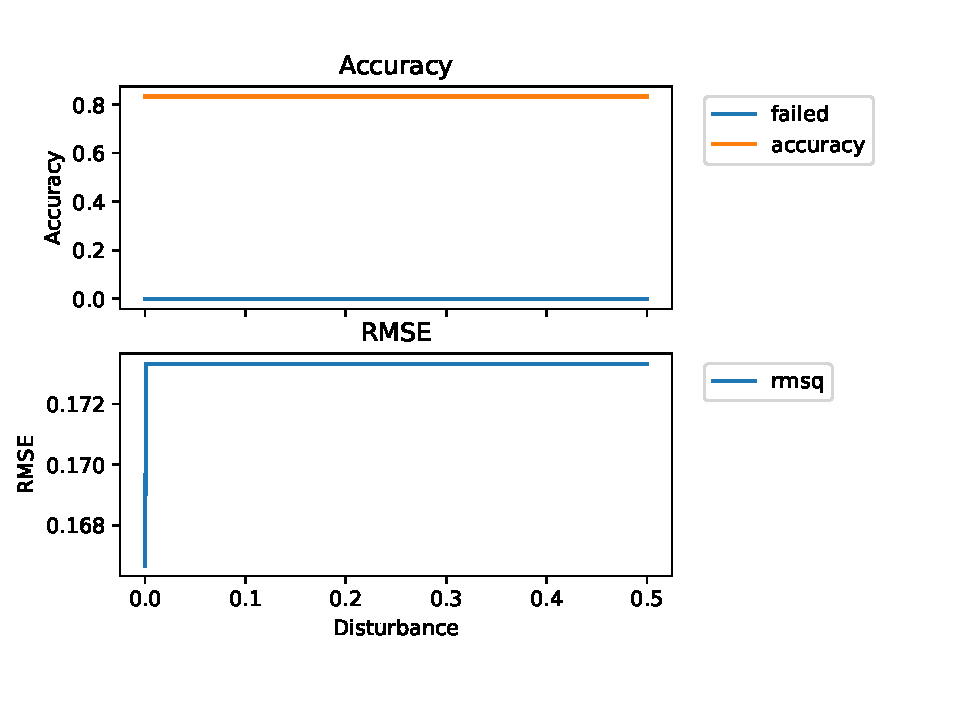
\includegraphics[width=0.9\linewidth]{../experiments/VlekNetwork/plots/performance_KB1.pdf}
\caption{Network 1 accuracy and RMS.}
\label{kb2a1}
\end{subfigure}%
\begin{subfigure}{.5\textwidth}
 \centering
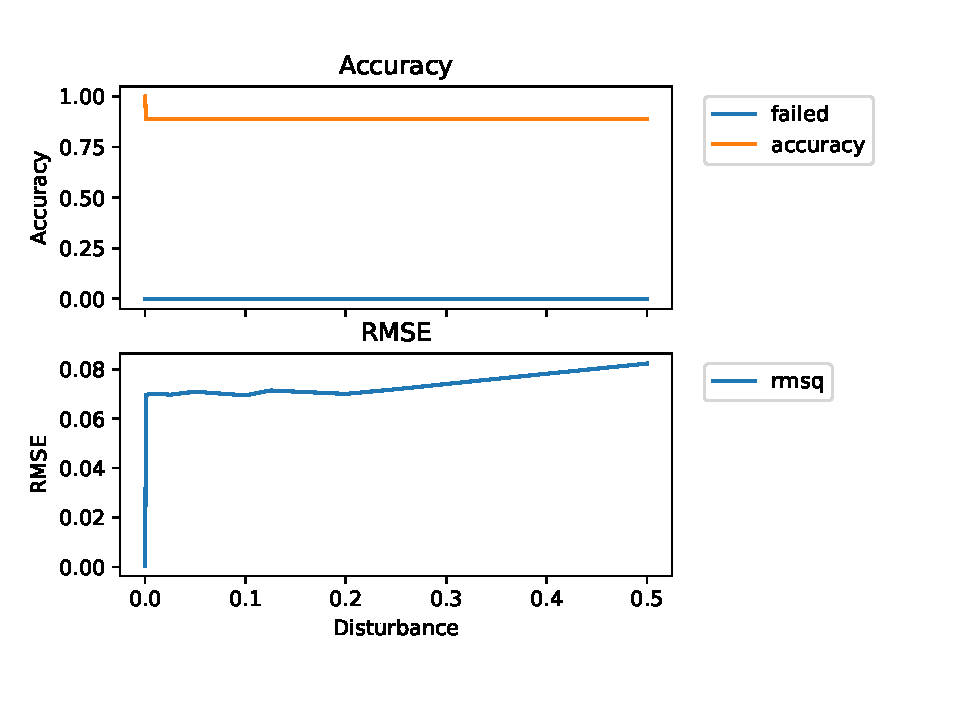
\includegraphics[width=0.9\linewidth]{../experiments/VlekNetwork/plots/performance_KB2.pdf}
\caption{Network 2 accuracy and RMS.}
\label{kb2p}
\end{subfigure}
\begin{subfigure}{.5\textwidth}
\centering
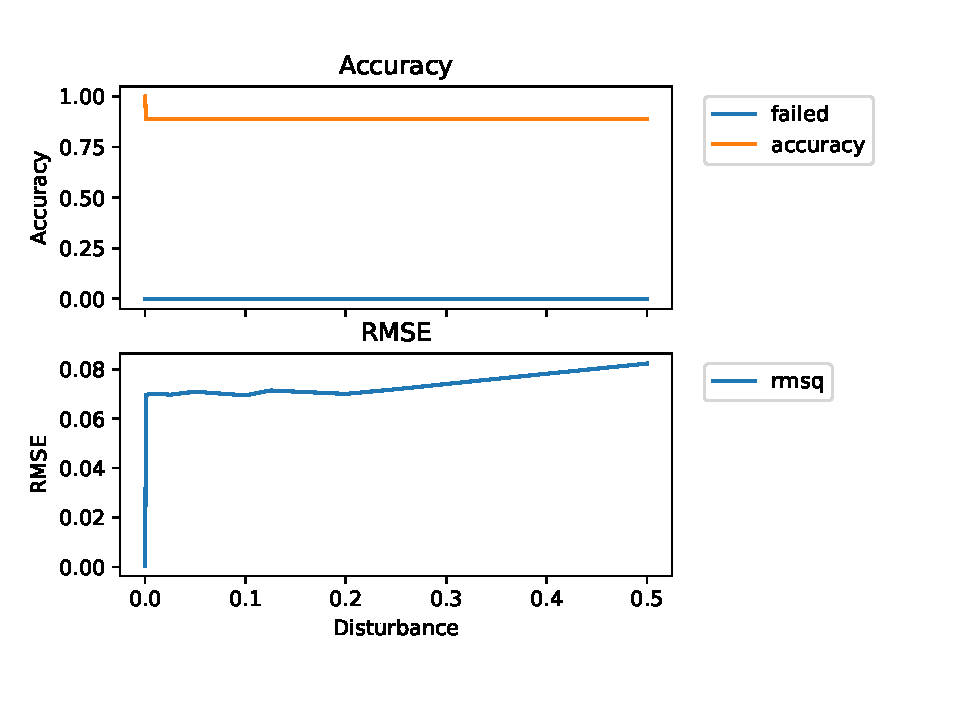
\includegraphics[width=0.9\linewidth]{../experiments/VlekNetwork/plots/performance_KB2.pdf}
\caption{Combined network accuracy and RMS.}
\label{fulla1}
\end{subfigure}%
\caption{Using error terms instead of 1 and 0 in the networks improves performance immensely.}
\label{error}
\end{figure}


\item \textbf{Could a human find these probabilities?}

Using the $\epsilon$-networks with lower precision, like rounding to 0.1, 0.25 or even 0.33, is a promising approach. Especially in cases where a node has multiple parents, being able to fill out probabilities to a lower precision is very useful. This low-precision approach also lends itself well to conversions to a verbal probability scale \citep{renooij1999}.

However, when you round the cpts to a lower precision, you are still rounding based on the original value. If you did not have the original value, would you be able to think of it? The original network has as prior probabilities for the $P(fight) = 0.2$, and $P(knife) = 0.7$. It is unclear how these values would be elicited from experts, if this were a real court case.

For one, how to operationalise these variables? We have it easy in our simulation `Jane has a knife' is true if and only if the reporter for `jane has a knife' is true, which is based on a random number generator. However, in real life, what do we mean? Do we mean all situations where Jane is in possession of a knife? A lot of these situations are not relevant, if Jane is an adult woman, she probably owns a knife in her kitchen, and we would say $P(jane\_has\_knife) = 1 -\epsilon$. If instead we mean that we consider all the situations where Jane has a knife within reach, we know that that that probability is going to be lower than $1-\epsilon$ - but out of all the possible `situations' that Jane can be in, we would consider that probability to be $\epsilon$: if we consider all seconds of your life and consider the proportion of those where you had a knife within reach, that would be a proportion smaller than $\epsilon = 0.01$. This is also not useful. 

If we cannot determine what reference class to take for `Jane has a knife', we might just give up and assign the node a probability of 0.5. This is what we do in the lowest-possible precision level, rounding everything to $\{\epsilon, 0.5 , 1-\epsilon\}$ - the resulting network still has a high accuracy. So in the case of these networks, it might actually be plausible to use Bayesian uncertainty priors.


\item \textbf{ Can a human determine the correct independence relations?}
These rounded networks are in-part accurate, because they are using the same structure as the original network. We do not have to derive the structure independently, based on no information. We already have the structural information based on the information from the simulation. Would you be able to derive this structure without using the simulation, or only while having limited information?

In case of scenario 1 and 2, certainly a person would be able to determine the correct independence relations: these scenario is very temporally ordered, and we see clear cause and effect. An additional relation between `jane\_and\_mark\_fight' and `jane\_has\_knife' might be appropriate, since, thinking naively, Jane might be more likely to have a knife if she knows that she and Mark have a history of fighting and/or violence. However, this is not modelled in the original scenario \citep{Vlek2015}, and hence not modelled in the simulation either.

The combined scenario, however, is more complicated. While there is some temporal organisation, since the parents of nodes usually occur before the nodes themselves, there are more arcs between nodes than in either of the two independent scenarios. The temporal organisation is also broken by the nodes `mark\_dies', which might happen after Mark threatening Jane, but is the parent of that node nonetheless (and the rest of that chain of events). A second atemporality occurs between the stabbing and threatening node (see discussion in Comparison below). 

Dependencies between Mark hitting Jane and Mark dying by accident should be irrelevant based on the events that could happen in between (like Jane dropping the knife, and Mark falling on the knife). Looking at the cpt of `mark\_dies\_accidentally', there are a lot of replicated values. It is unclear how the algorithm should be adapted to reduce the amount of unnecessary dependencies.
\end{enumerate}


\section{Discussion}
In the discussion, we focus on the comparison of the automatically generated networks to the paper in Vlek, and consider some other issues.


\subsection{Comparison to Vlek's Method}

The Bayesian Networks generated using the method outlined in this paper diverge meaningfully from the networks as presented in \citet{Vlek2015}. 

Firstly, in the original paper there was no integration of both scenarios into one network. In this paper, the combination is shown in Figure~\ref{full}. For the integration of two scenarios, Vlek proposed combining the networks from Figure~\ref{kb1} and Figure~\ref{kb2} using the merged scenario idiom construction as outlined in \citet{Vlek2014}. This merging depends on a scenario-like construction with a constraint node, and requires extra probabilities to be elicited. In this case, there was no `merging' of two networks, instead the simulation was run with all the rules and reporters (and one excluding rule that states that if Jane was threatening Mark, Jane couldn't stab Mark). In short, the `merging' happened at the simulation level, and the data obtained from the simulation was then used to create the network that combines both scenarios (Figure~\ref{full}), effectively effortlessly combining two networks.

Secondly, the network structure between the networks in \citet{Vlek2015} and this paper are different. In this case, there is no scenario node or subscenario-structure organisation. The only organisation in the automatically generated networks is the `temporal' structure of parent vs child nodes, which is usually present (the child event happens after the parent event). The subscenario-structure we see in Figure~\ref{vlek} is not present. The lack of scenario, subscenario and constraint nodes, is because these are not necessary in representing the events of the simulation. A `scenario' is not ordered using a scenario node, but instead should be modelled in such a way that when setting evidence, some nodes being true `cause' other nodes to become false (and vice versa). The scenarios, in this project, emerge from the network, instead of being represented explicitly.

The temporal structure is not consistently present in the networks, however. In Figure~4.3, we see that the node `mark\_dies' is the parent node of almost all the nodes of the second scenario. This is because the temporal ordering in K2 is not straightforward when multiple scenarios are combined (eg, Mark dies after being stabbed, which is the 4th and final event in scenario 1, but Mark can also die after falling on the knife, which is the 6th event in scenario 2). Either improving the temporal ordering algorithm or the ordering of nodes by the modeller could improve this situation. 

Even though the networks in this paper are different from the networks in \citet{Vlek2015}, we can still use the criteria of completeness, consistency and plausibility outlined in that work to assess their quality.

\begin{itemize}
\item Completeness can be operationalised in this situation, not by looking at story schemes and idioms, but by looking at the reporters in the simulation. A network can be considered complete if it represents every reporter as a node. This means that all the networks are complete, because every network contains nodes that correspond to all reporters. It is more likely that we suffer from the opposite problem, where irrelevant reporters are still included in the network. 

\item Consistency means that there are no internal contradiction. In this network, consistency cannot be seen structurally (by separate scenarios and constraint nodes). The node `jane threatens mark with knife' and the node 'jane stabs mark with knife' are inconsistent, but they belong in the same network. Instead of structurally, consistency is ensured using the conditional probability tables. The relations of these nodes are such, that when one is true, the other becomes false (Figure~\ref{cont}).


This means that several different scenarios can be combined into one network, while the overall network is still consistent. Both scenarios share some events (as scenarios can do in real life), but the different scenarios themselves are not separated from each other by structure, and we do not need the constraint node as suggested in \citet{Fenton2011}. Fenton suggests two objections against a solution as presented here: unnecessary extra numbers, and lack of causal interpretation. Unnecessary extra numbers is not a problem here, because we do not need to elicit them (they fall out of the algorithm automatically). For causality, we are not interpreting the arcs between nodes causally in any way. They are conditional, and in that case it does not matter which node is the parent.

Other types of inconsistency - such as Jane stabbing Mark, when Jane does not have a knife, result in a `conflict' message when when the network is imported into Hugin. PyAgrum does not show such a conflict message.

\begin{figure}[htbp]
\begin{subfigure}{.3\textwidth}
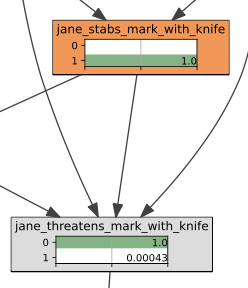
\includegraphics[scale=0.5]{images/vlekprog/e1.png}
\caption{Stabbing means no threatening.}
\label{e1}
\end{subfigure}
\begin{subfigure}{.3\textwidth}
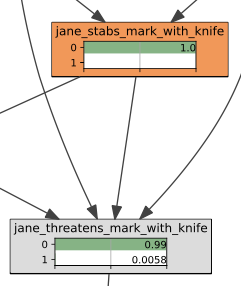
\includegraphics[scale=0.5]{images/vlekprog/e2.png}
\caption{Not stabbing does \textbf{not} mean that there's threatening, we do not have mutual exclusivity constraint.}
\label{e2}
\end{subfigure}
\begin{subfigure}{.3\textwidth}
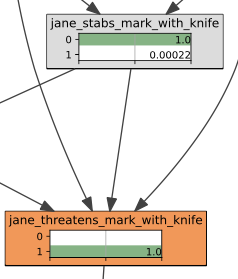
\includegraphics[scale=0.5]{images/vlekprog/e3.png}
\caption{Threatening with knife means that there's no stabbing.}
\label{e3}
\end{subfigure}
\caption{Effect of setting evidence on contradictory nodes.}
\label{cont}
\end{figure}

\item Plausible. Plausibility is defined such that a scenario should correspond to the modellers knowledge about the world. In this case, we have outsourced the problem of plausibility to the simulation, and the Bayesian Network reflects it. 

If we set to true one of the nodes in the temporal chain that leads towards the outcome of scenario 2, then we find that the rest of the nodes in that chain become more plausible - but not by much, because scenario 2 is very implausible to begin with! For example, P( `mark\_falls\_on\_knife' $| \emptyset$) = 0.00028, but once we know that Jane has threatened Mark, we see P( `mark\_falls\_on\_knife' $|$ `jane\_threatens\_mark\_with\_knife) = 0.046. Implausible elements become more plausible once we find support for them, reflecting the modeller's knowledge about the world.

\end{itemize}
%\textbf{Do we need the constraint node? }

%We can just  draw a line between two events in order for them to become mutually exclusive, like we do with `Jane stabs mark' and `jane threatens mark'. Fenton et al advice against that - we draw a relation between two causes to ensure mutual exclusivity. Fenton doesn't like this even though it satisfies the axioms he sets out in the paper because 1) the parent cause becomes part of the causal pathway leading to the child cause, which means that you have to involve many more numbers (``meaningless columns''). Fortunately, this is not a problem in the automatically generated BNs, because the algorithm fixes this for us :). Not sure if an extra node is good for the computational complexity of BNs either. Uh. Anyway, even if this is not the case, there are lots of unnecessary numbers in Bayesian Networks anyway, because there's many combinations of events that just do not happen (eg: mark dies but jane doesn't have a knife, never happens, but is in the table anyway. Unnecessary complexity? Probably a rounding error!!). Anyway, that's a thing. So it doesn't really matter.

%The second objection to using the direct connection over the constraint node is that you have to arbitrarily decide which cause is the parent - which doesn't make sense if you interpret the networks causally. Fortunately. there's no causality in this part, its just frequencies and conditional probabilities, so it doesn't matter, we can just pick one and it's fine. So turns out we don't need the constraint node anyway :D



So our overall conclusion with regards to the quality of the network, is that the networks represent the scenarios well with regards to completeness, consistency and plausibility, even without structural support from scenario, sub-scenario and constraint nodes. This means that this method seems promising and does not need to include or build on the scenario-type structures.

\subsection{Further Discussion}


\subsubsection{Are we just outsourcing?}

This approach to completeness and plausibility outsources the problem of determining completeness or eliciting plausibility from the builder of the network to the builder of the simulation. We get a complete network for free, given a simulation, in our approach, but that is because we are basing our network entirely on the simulation. This brings up the following problem: what does it mean for a simulation to be `incomplete'? How can we know that the probabilities inputted in the simulation are plausible?

 There is no good answer to this question. A simulation will always be an incomplete reflection of reality. Perhaps the simulation should correspond to some story or idiom. If the scenario contains `intentional' agents, we might find it easier to think about stories and idioms in simulation than we find it to think about stories and idioms with regards to Bayesian Networks. However, this needs to be investigated further.
 
 \subsubsection{Bayesian Networks as a guide to reasoning}
 Ideally, we would want a BN to protest when you try to add evidence to it that corresponds to an impossible world state. This should cause conflict between nodes, or at least result in a low accuracy. We calculated accuracy over the set of all possible world states, however, if we take the accuracy over the set of all impossible world states (eg: states that never occur in the simulation), we would want to see a low accuracy. So, the accuracy over the impossible world states is shown in Table~\ref{tabVlekNetworkimpossible} , shows for the generated $\epsilon$-networks.
 \begin{table}[htp]
\begin{center}
\begin{tabular}{|c|c|c|c|}
 \hline
 Network & Accuracy & Root Mean Square & Inconsistency error\\
 \hline
 Scenario 1   & 0.3 &  0.70 & 0   \\
 Scenario 2 & 0.481 & 0.516 & 0\\
 Combined & 0.491 & 0.509& 0\\
\hline
\end{tabular}
\caption{Accuracy and Root Mean Square Error for the networks calculated on the impossible states.}
\label{tabVlekNetworkimpossible}
\end{center}
\end{table}

Here, the accuracy is remarkably low, and the RMSE is high. This means that if you, by accident, fill in an impossible world state as evidence in your BN, the probability that you predict the output node correctly becomes very low. However, we also see that these $\epsilon$-networks do not break - the number of times that we find an inconsistency error is 0 for all networks. In the best case scenario, we want the network to break if you fill in inconsistent evidence, and not just produce a low accuracy (since you can only calculate accuracy over a data set). 


\subsubsection{Resolution and number of runs}
The accuracy of the Bayesian Network improves as the number of runs improves. This is an obvious fact. It has implications for the rest of the network. For example, if we run the network too few times (let's say 10 times), then the network will not be able to estimate the probability of certain states - eg: the probability that Mark hits Jane can be calculated as: $0.7 \cdot 0.2 \cdot 0.03 \cdot 0.9 = 0.00379$, which means that there's a 0.378\% chance that it happens, eg, if we run the simulation a 1000 times, Mark will hit Jane in 4 of them (or, actually, the sentence ``Mark hits Jane" is true in 4 of them). If we go all the way down the chain of unreasonable facts to ``Mark dies accidentally", we get a probability of 0.0001134, which is 1 every 10.000 runs. If we run the simulation 10.000 times, that means that we cannot estimate probabilities that are smaller than 0.0001 - either they occur `accidentally', eg, by chance, and the network estimates that they happen once every 10.000 runs, or they don't happen within 10.000 runs, and the network estimates that these events never happen at all - when in fact, they might happen, but just once every 20.000 runs.

What are the practical implications of this? On this side, that we need enough data to get an accurate prediction. But, if we're thinking about elicitation, this means that if you decide to add an event to a scenario, or a node to a network, you really have to think about the probability that you assign it - a probability of 1 in 10.000 would really mean that this event would only happen once every 10.000 situations.

\subsubsection{Future Research}
This simulation and network are actually not a good representation of agent-based modelling. There are no agents acting with intentions or beliefs or knowledge, it's just a global forward-chaining engine firing off a rule when a random number generator says that it can. There was no emergence of probabilities due to interactions of agents with their environment, or with each other. This type of emergent behaviour and intention is essential for modelling crime cases, and will be introduced in the next chapter.

There were also no separate evidence nodes, because the original networks and scenarios did not contain evidence. Evidence will also be introduced in the next chapter.



\subsection{Conclusion}
Even this very simple `forward chaining' simulation (forward chaining with some probabilities attached), can be used to construct meaningful Bayesian Networks. The generated Bayesian Networks have generally high accuracy and low RMS error, even when their cpts are disturbed,  when we use an error term instead of 0. The Bayesian Networks reflect the structure of the simulation. 

This shows the success of the pipeline. We can make a simulation using forward chaining, that generates world-states, and those world states can be translated into Bayesian Networks by means of the K2 algorithm, with reasonable accuracy even under decreased precision. The K2 manages to replicate constraints and merge two different possible scenarios together. The resulting networks are consistent, complete and plausible. The scenario, sub-scenario and constraint node mechanisms are not necessary for modelling these Bayesian Networks.

So if the real world worked like a simple forward chaining inference method where we knew exactly when a proposition was true (which is, if the state is true, we set the proposition to true in every epoch), then BNs would work flawlessly, even if we weren't very great at estimating the correct frequencies precisely.



%> Dit is de focus van mijn onderzoek!!!

%> ik laat zien welke dingen je allemaal nodig hebt om statistische shit te gebruiken
%> als een van deze dingen niet aanwezig is, is het dus niet mogelijk om BNs te gebruiken in het echt
%> in de simulaties weet je precies welke wetmatigeheden je hebt (want die definieer je met je simulatie/forward chaining etc)
% s> maar die kunnen we dus nooit in het echt vinden. En dus kunnen we BNs nooit in het echt toepassen. end.


